\documentclass{beamer}
\setbeamertemplate{navigation symbols}{}
\setbeamertemplate{itemize items}[ball]
\usetheme{default}
\usecolortheme{seahorse}
\usepackage[]{algorithm2e}
%\setbeamertemplate{navigation symbols}{}
\beamersetuncovermixins{\opaqueness<1>{25}}{\opaqueness<2->{15}}
\begin{document}
\title{Community-based semantic subgroup discovery}
\subtitle{(CBSSD)}
\author{Bla\v{z} \v{S}krlj, An\v{z}e Vavpeti\v{c}, Jan Kralj, Nada Lavra\v{c}}
\date{\today} 

\usebackgroundtemplate{%
  
\includegraphics[width=\paperwidth,height=\paperheight]{images/header}}

\begin{frame}

  {
    \usebackgroundtemplate{
\includegraphics[width=\paperwidth]{images/header.png}}%
    \titlepage
    
  }
  
\end{frame}

\usebackgroundtemplate{%
  
\includegraphics[width=\paperwidth,height=\paperheight]{images/background}}

\begin{frame}\frametitle{Table of contents}\tableofcontents
\end{frame}


\section{General overview} 

\begin{frame}\frametitle{Introduction} 


  \begin{columns}
    \begin{column}{0.5\textwidth}

  \begin{block}{Properties of biological networks}
    \begin{itemize}

    \item Multiple types of nodes and edges $\rightarrow$ heterogenous networks
    \item Possible connections between distinct entities
    \item Large in some sub-domains
    \item Not trivial to interpret
      
    \end{itemize}
  \end{block}
      \end{column}
    \begin{column}{0.5\textwidth}  %%<--- here
      \begin{center}
        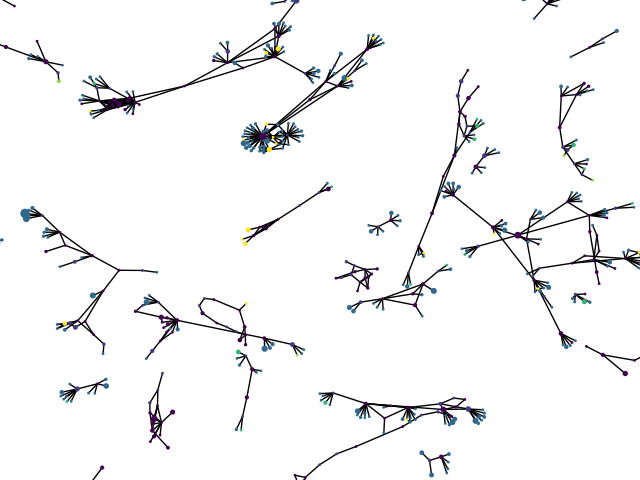
\includegraphics[width=1\textwidth]{images/figure_2}
      \end{center}
    \end{column}
    \end{columns}
  \end{frame}

  \begin{frame}\frametitle{How can an algorithm learn from a complex network?}

    \begin{block}{Network representation}
      Important network features can be encaptured via community detection, graphlets, semantic clustering and other methods..
    \end{block}

    \begin{exampleblock}{Example use}
      Such methodology is used to infer protein-RNA interactions, identify expression patterns, compare protein structures, fuse systems-level data etc.
    \end{exampleblock}
    
  \end{frame}
  
\section{Problem definition} 
  \begin{frame}\frametitle{Problem definition}

    \begin{block}{Term-subset enrichment}
      Let ${t_{1},t_{2},..,t_{n}}$ represent individual terms of interest from the whole term set $\psi $. Identify subsets $\Lambda_{1},\Lambda_{2},..,\Lambda_{n} \subseteq \psi$, which represent interpretable patterns, previously unknown to a human observer.      
    \end{block}

    \begin{exampleblock}{Example situation}

      Let $G_{1},G_{2},..,G_{n}$ be $n$ distinct genes we are interested in. Although individual genes, or the whole group of genes doesn't return any interesting results, we can further explore the subspace of n genes.

    \end{exampleblock}
    \begin{alertblock}{Problem}
      Exploring all possible combinations can be computationally expensive procedure, as there are $\sum_{i=2}^{n}\dfrac{n!}{(n-i)!i!}$ possible options.      
    \end{alertblock}      
  \end{frame}

\section{Proposed approach}
  \begin{frame}\frametitle{Fighting the combinatorial explosion}

    We argue there exists an efficient heuristic-based approach.
      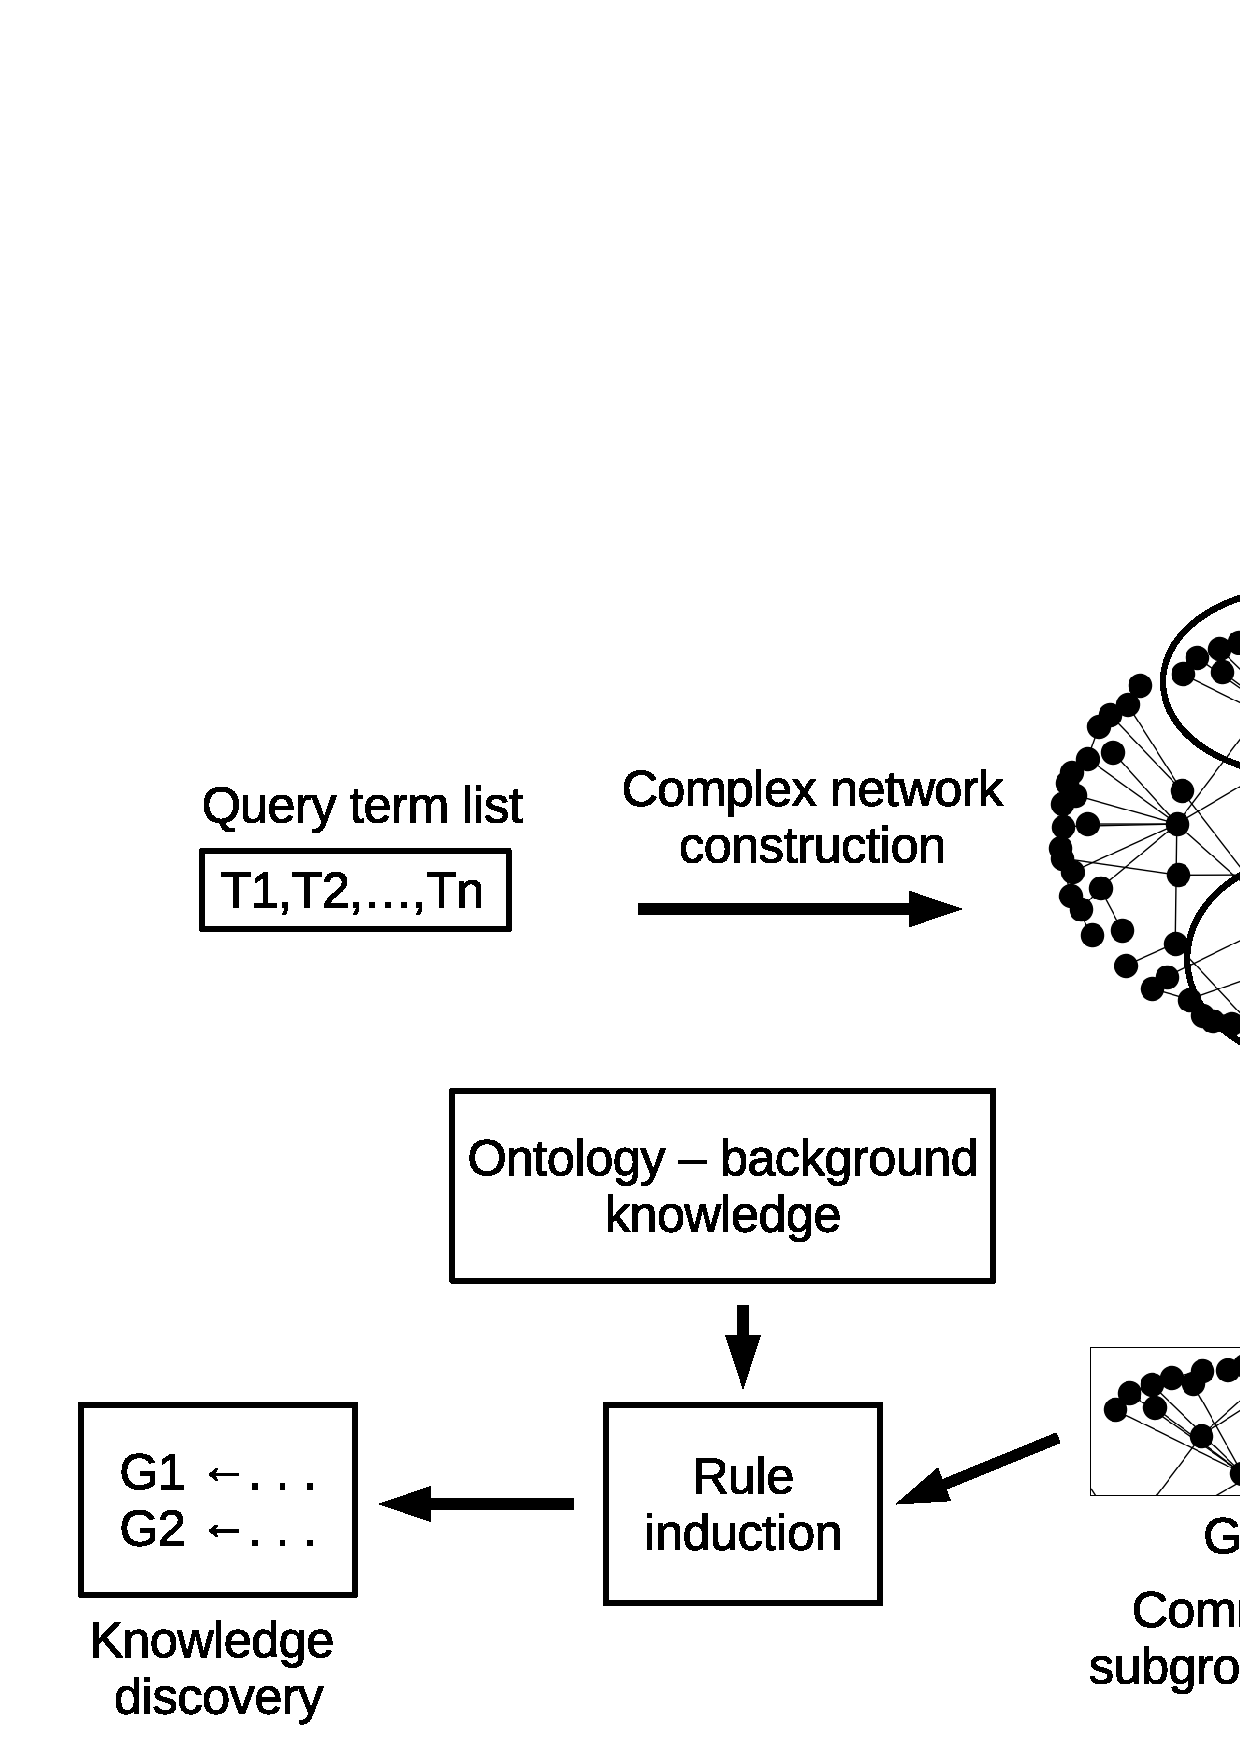
\includegraphics[scale=0.35]{images/workflow2}       
   \end{frame}

  \begin{frame}\frametitle{Fighting the combinatorial explosion - network construction}



  \begin{columns}
    \begin{column}{0.5\textwidth}


      \begin{block}{Basic procedure}
      \begin{itemize}
      \item collect network data on the studied phenomenon
      \item merge the data into a single heterognous network
      \item simplify the obtained network        
      \end{itemize}

      
      \end{block}
      
      \end{column}
      \begin{column}{0.5\textwidth}  %%<--- here
        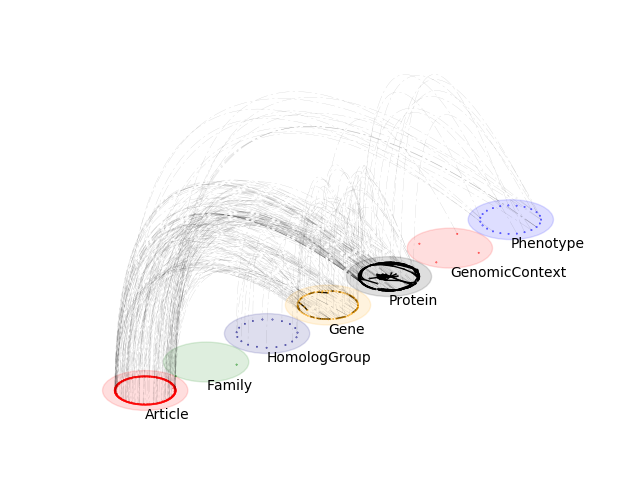
\includegraphics[scale=0.35]{images/figure_1}
      \end{column}
      
    \end{columns}
    
   \end{frame}


   
\end{document}